\documentclass[problems]{esg8022pset} 
  \usepackage{amsmath}
  \usepackage{amssymb}
  \usepackage{enumerate}
  \usepackage{graphicx}
  \usepackage{hyperref}
  \usepackage{mathtools}
  \usepackage[per-mode=symbol]{siunitx} %If this line is giving you trouble, try replacing per-mode with per
  \providecommand{\uvec}[1]{{\hat{\bf{#1}}}}
  \usepackage{pgf,tikz}
  \usetikzlibrary{arrows}
  \usepackage{wasysym}
  \makeatletter
  \newcommand{\interitemtext}[1]{%
    \begin{list}{}
     {\itemindent=0mm\labelsep=0mm
     \labelwidth=0mm\leftmargin=0mm
     \addtolength{\leftmargin}{-\@totalleftmargin}}
      \item #1
    \end{list}
  }
  \makeatother
  \renewcommand{\d}{\,d}
  \providecommand{\norm}[1]{\lVert#1\rVert}
\classname{Physics 8.022} \semester{Spring 2011} 
\problemsetnumber{2} 
\date{\today } 
\duedate{Sunday, February 13} 
\readingassignment{} 
\psettitle{Gauss's law and electric potential} 
\begin{document}
  \addtocounter{section}{-1}
\section{Problem \thesection: Line integrals; work; units and dimensional analysis (Optional)}
  A force ${\vec F} = A(y^2{\hat x} + 2x^2{\hat y})$ is acting on a
  particle which is initially at the origin of the $(x,y)$ coordinate
  system.  We transport the particle on a square path defined by the
  points $(0,0)$, $(0,l)$, $(l,l)$, $(l,0)$, $(0,0)$.  The constant $A$
  is positive.

  \begin{enumerate}[(a)]
    \item Suppose we work in SI units: the coordinates $(x,y)$ are measured
      in meters, so that the particle moves $l$ meters along each leg of the
      path; the force is measured in Newtons.  What must be the units of
      $A$?  Express in terms of kg, m, and s.
    \item Suppose we work in cgs units: the coordinates $(x,y)$ are measured
      in centimeters, and the force is measured in dynes.  What must be the
      units of $A$?  Express in terms of gm, cm, and s.
    \item How much work does the force do when the particle travels around
      the path?  (Your answer does not depend on the choice of units:
      express it in terms of the constants $A$ and $l$, which are assumed to
      have units built into them.)  Is this a conservative force?
    \item If we place a particle right at the origin, the total force is
      zero, so it will just stay there.  Is this a stable situation?  Give
      any argument you please (mathematical, physical, intuitive) to justify
      the stability (or instability) of this situation.
  \end{enumerate}
\section{Problem \thesection: Purcell 1.16}
  The sphere of radius $a$ was filled with positive charge at uniform density $\rho$. Then a smaller sphere of radius $a/2$ was carved out, as shown in the figure, and left empty. What are the direction and magnitude of the electric field at $A$? At $B$?
  \begin{center}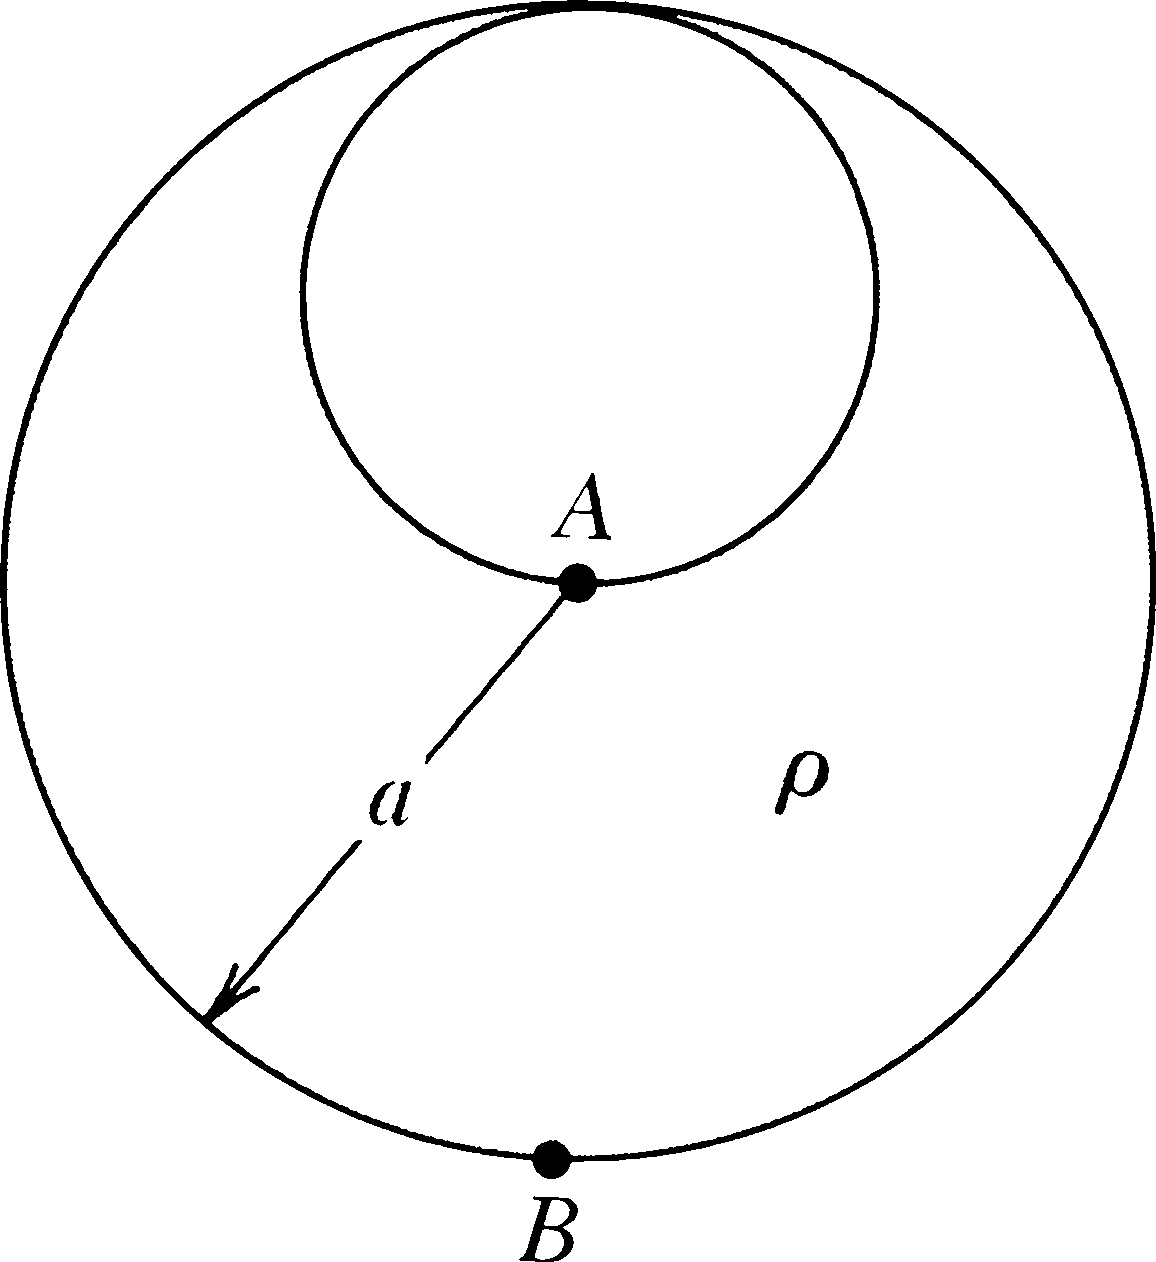
\includegraphics[width=0.3\textwidth]{ps02_1}\end{center}
\section{Problem \thesection: Purcell 1.17}
  \begin{enumerate}[(a)]
    \item A point charge $q$ is located at the center of a cube of edge length $d$. What is the value of $\int \vec E \cdot d\vec a$ over one face of the cube?
    \item The charge $q$ is moved to one corner of the cube. What is now the value of the flux of $\vec E$ through each of the faces of the cube?
  \end{enumerate}
\section{Problem \thesection: Purcell 1.31}
  A charged soap bubble experiences an outward electrical force on every bit of its surface. Given the total charge $Q$ on a bubble of radius $R$, what is the magnitude of the resultant force tending to pull any hemispherical half of the bubble away from the other half? (Should this force divided by $2\pi R$ exceed the surface tension of the soap film interesting behavior might be expected!)

  \begin{flushright}\emph{Ans}. $Q^2/8R^2$.\end{flushright}
\section{Problem \thesection: Purcell 2.1}
  The vector function which follows represents a possible electrostatic field:

  \begin{align*}
    E_x & = 6xy &
      E_y & = 3x^2 - 3y^2 &
        E_z & = 0
  \end{align*}

  Calculate the line integral of $\vec E$ from the point $(0, 0, 0)$ to the point $(x_1, y_1, 0)$ along the path which runs straight from $(0, 0, 0)$ to $(x_1, 0, 0)$ and thence to $(x_1, y_1, 0)$. Make a similar calculation for the path which runs along the other two sides of the rectangle, via the point $(0, y_1, 0)$. You ought to get the same answer if the assertion above is true. Now you have the potential function $\phi(x, y, z)$. Take the gradient of this function and see that you get back the components of the given field.
\section{Problem \thesection: Purcell 2.4}
  Describe the electric field that goes with the following potential:
  \begin{align*}
    \phi & = x^2 + y^2 + z^2 & \text{for }x^2 + y^2 + z^2 < a^2 \\
    \phi & = -a^2 + \frac{2a^3}{(x^2 + y^2 + z^2)^{1/2}} & \text{for }a^2 < x^2 + y^2 + z^2
  \end{align*}
  Discuss what happens at the boundary ($x^2 + y^2 + z^2 = a^2$).
\section{Problem \thesection: Purcell 2.8}
  For the cylinder of uniform charge density in Fig. 2.17:
  \begin{enumerate}[(a)]
    \item Show that the expression there given for the field inside the cylinder follows from Gauss's law.
    \item Find the potential $\phi$ as a function of $r$, both inside and outside the cylinder, taking $\phi = 0$ at $r = 0$.
  \end{enumerate}
  \begin{center}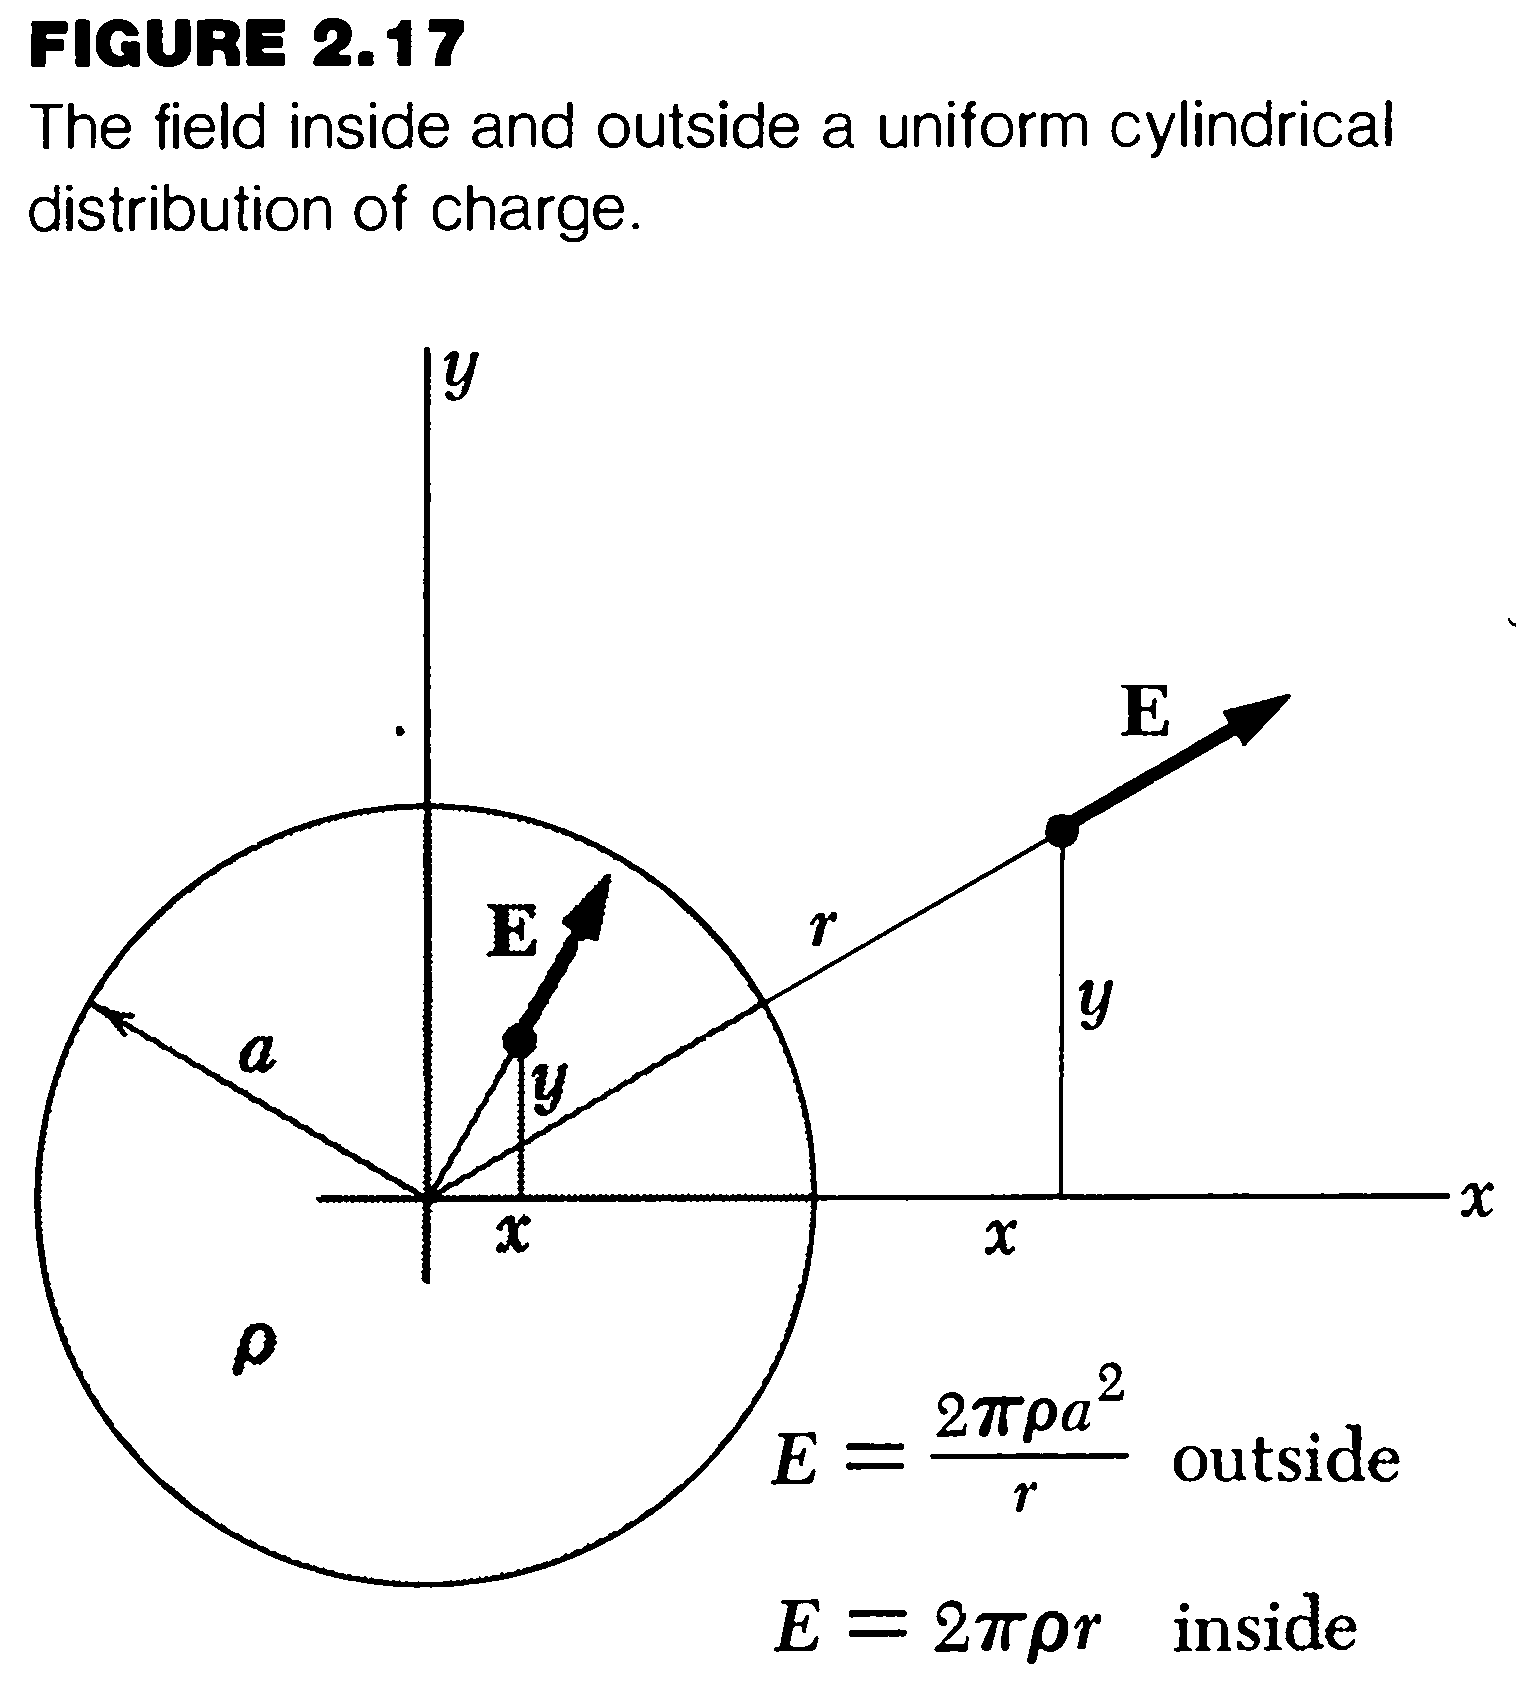
\includegraphics[width=0.4\textwidth]{ps02_2}\end{center}
\section{Problem \thesection: Purcell 2.12}
  The right triangle with vertex $P$ at the origin, base $b$, and altitude $a$ has a uniform density of surface charge $\sigma$. Determine the potential at the vertex $P$. First find the contribution of the vertical strip of width $dx$ at $x$. Show that the potential at $P$ can be written as $\phi_P = \sigma b \ln[(1 + \sin \theta) / \cos \theta]$.
  \begin{center}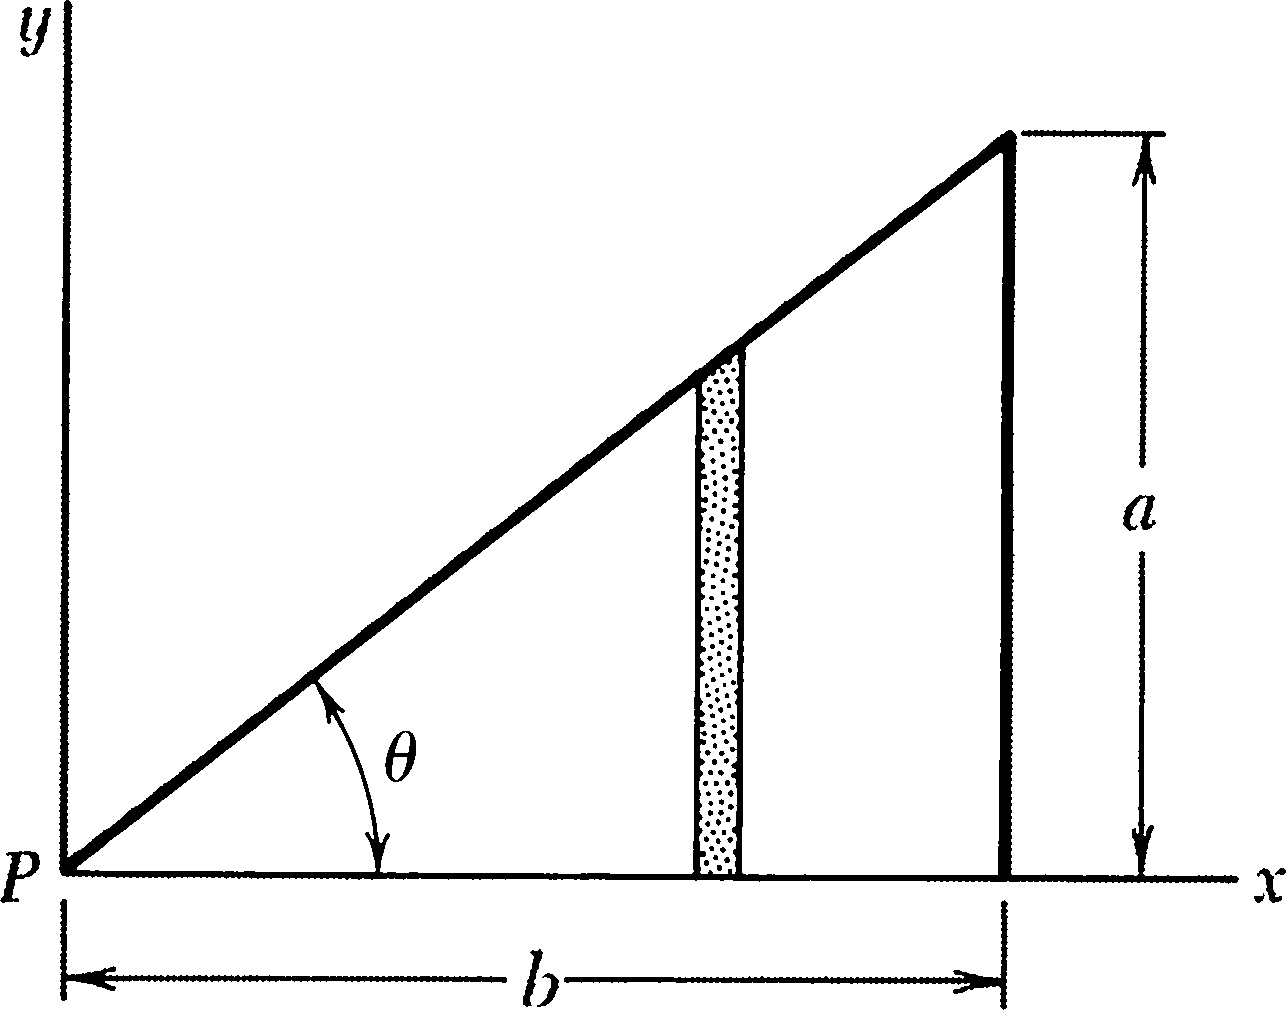
\includegraphics[width=0.35\textwidth]{ps02_3}\end{center}
\section{Problem \thesection: Purcell 2.30}
  Consider a charge distribution which has the constant density $\rho$ everywhere inside a cube of edge $b$ and is zero everywhere outside that cube. Letting the electric potential $\phi$ be zero at infinite distance from the cube of charge, denote by $\phi_0$ the potential at the center of the cube and $\phi_1$ the potential at a corner of the cube. Determine the ratio $\phi_0/\phi_1$. The answer can be found with very little calculation by combining a dimensional argument with superposition. (Think about the potential at the center of a cube with the same charge density and with twice the edge length.)
\end{document}
